One would like to collect as much light as emitted from the scintillator as possible.
In practice two effects limit the fraction of the emitted light collected; the optical self-absorption in the material and losses at the edges of the optical surfaces \cite{knoll_radiation_2009}.
The optical self-absorption of a scintillator is a material property in which photons are reabsorbed by the material.
This effect is important for large area scintillators and for scintillators which are not optically  clear, both of which apply to the developed polymeric scintillators.
Typically this effect is mitigated by the use of a wavelength shifting fiber in which the light is transferred to a material which has a much lower optical self-absorption.

Light collection of a scintillation event is emitted isotropically, and therefore only a very small fraction of the photons can travel directly to a photon detector surface.
The majority of the light must then be collected by reflecting back into the medium.
Snell's law governs the reflection of light at an optical boundary, and there are two cases to consider as shown in \autoref{fig:SnellsLaw} and described by Snell's Law, \eqref{eqn:SnellsLaw}
\begin{align}
	\theta_c = \sin^-1 \frac{n_1}{n_0}
	\label{eqn:SnellsLaw}
\end{align}
where \definevar{$\theta_c$}{critical angle}, \definevar{$n_1$}{index of refraction of the surrounding medium} and \definevar{$n_0$}{index of refraction of the scintillator}.
If the angle of incidence, $\theta$, is greater than the critical angle total internal reflection will occur.
When the angle of incidence is less than the critical angle particle reflection (or \textit{Fresnel} reflection) will occur and there will be partial transmission of the photons to the surrounding medium.
\begin{figure}
	\centering
	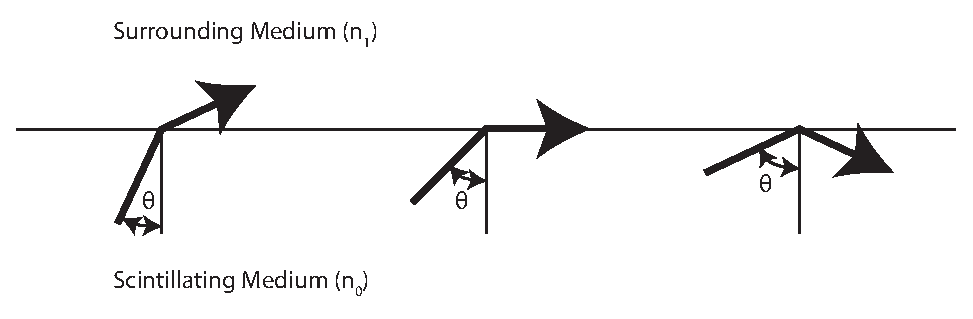
\includegraphics[width=\textwidth]{LightBoundary_SnellsLaw}
	\caption[Light Reflection at a Boundary]{Reflection of light at an optical surface is governed by Snell's law.  The fraction of light reflected back into the material is greatest at an angle of incident equal to $\theta_c$}
	\label{fig:SnellsLaw}
\end{figure}
To ensure that the light stays within the desired medium it is usually encased in a reflector, of which there are two types (\autoref{fig:SpecularDiffusive}).
A polished metallic surface (such as aluminized mylar) may be applied as a specular reflector which are generally better when the length is much longer than the thickness\cite{SaintGobain_DAM_2012}.
A diffusive reflector, such as teflon tape, is better for conditions when the detector is thick compared to its length \cite{knoll_radiation_2009}.
\begin{figure}
	\centering
	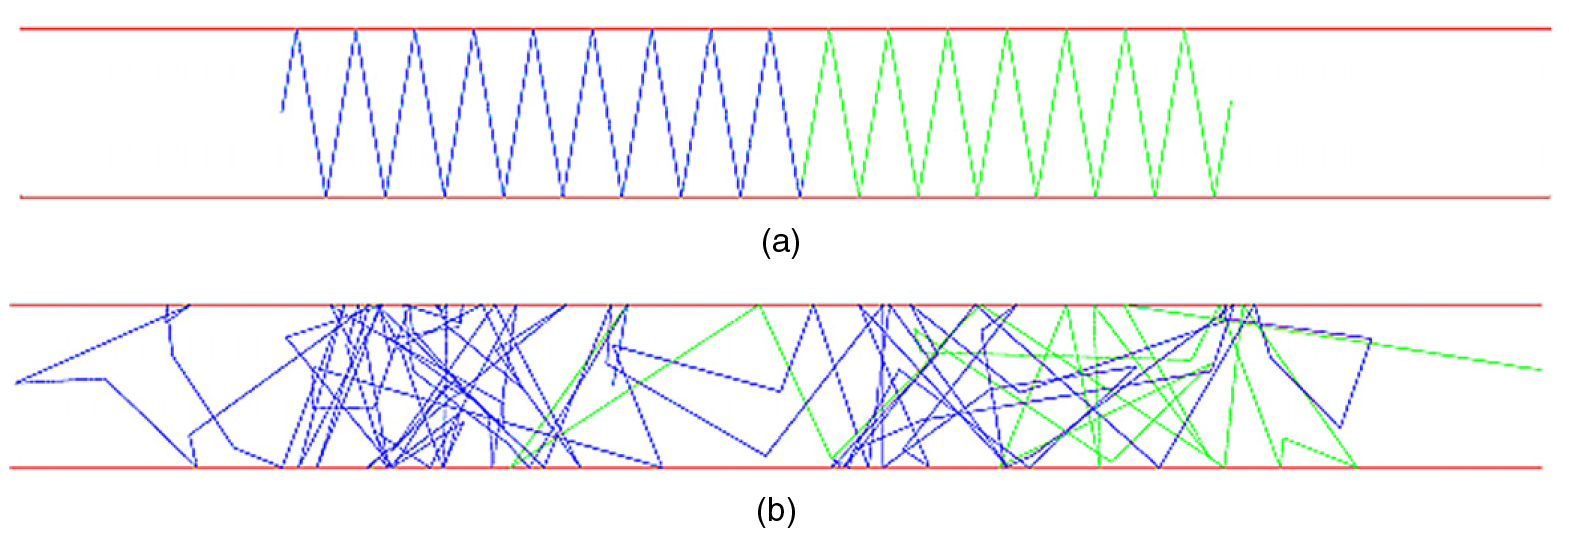
\includegraphics[width=\textwidth]{Riggi_SpecularDiffusive}
	\caption[Specular and Diffusive Reflection]{Specular reflection (a) in which the light in a single incoming direction is emitted as a single outgoing direction. The rough surface of a diffusive reflector (b), causes the light to be reflected at many angles. Figure from \cite{riggi_introducing_2011}.}
	\label{fig:SpecularDiffusive} 
\end{figure}
It should be noted, however, that one would like to optically match the surface at which the scintillator is to be viewed to prevent reflection.

Photons that are emitted exactly along the direction of the scintillator will only be effected by the  absorption length of the material (typically on the order of \SI{100}{\cm} to \SI{400}{\cm} \cite{SG_PlasticScint_2008}) while photons emitted in directions nearly normal to the direction of the scintillator will need to undergo thousands of reflections in order reach the PMT, which can double the length the photons must travel.
For perfect specular reflection it has been shown through simulation the the number of photons throughout a scintillating strip is only reduced by the optical absorption in that strip \cite{riggi_introducing_2011}.
In a realistic scintillator with a diffusive reflector the number of photons decreases by a factor of more than 10 \SI{50}{\cm} from the origination of the photon\cite{riggi_introducing_2011}.

In the cases of a large scintillating detector, such as the one presented in this work, it  may be necessary to employ more than one PMT to collect the light.
In such cases the use of light pipes may enhance the collection efficiency. 
Light pipes are not without costs, however, as they are generally of a high index of refraction to maintain a high internal reflection

The magnitude of the difficulty of collecting the optical photons is illustrated in \autoref{tab:PointSrcScintSlabResults}.
The simulation is a slab of EJ-200 \SI{200}{\cm} long, \SI{30}{\cm} wide, and of thickness between \SI{100}{\um} to \SI{1}{\cm} with perfectly polished sides so that the only interactions will be specular reflection due to Snell's law.
While this simulation is not entirely representative of the light production (a uniform volumetric distribution would more accurately reflect the production in the scintillator) and the boundary conditions (perfectly smooth, polished surfaces are unrealistic), it demonstrates that there is a large hit in the light collection due to having a thin detector.
It is also observed for the thin films that the distance from the PMT to the origination of the light has little effect as the rays need to start out nearly perpendicular to the PMT surface.
\begin{table}
	\caption[Fraction of Photons Detected from a Point Source on a single PMT]{Fraction of photons detected on a single PMT in a slab of various thickness from a point source located \SI{25}{\cm} and \Si{50}{\cm} from the detector.  The optical properties simulated are of that of EJ-200, with an optical attenuation length set to \SI{200}{\cm}.}
	\label{tab:PointSrcScintSlabResults}
	% Data for this table may be found on pg. 30 of the third lab notebook
	\begin{tabular}{c | c  c}
	\toprule
	Slab Thickness & Fraction Collected (\SI{50}{\cm}) & Fraction Collected (\SI{25}{\cm}) \\
	\midrule
	\SI{100}{\um} & 1.1\% & 1.1\% \\
	\SI{220}{\um} & 1.3\% & 1.7\% \\
	\SI{460}{\um} & 1.5\% & 1.9\% \\
	\SI{1}{\mm} & 2.2\% & 2.8\% \\
	\SI{2.2}[\mm} & 3.5\% & 4.2\% \\
	\SI{4.6}{\mm} & 5.1\% & 6.2\% \\
	\SI{1}{\cm} & 6.3\% & 7.3 \% \\
	\bottomrule
	\end{tabular}
\end{table}
